\documentclass{article}

\usepackage[utf8]{inputenc}

\usepackage{amsmath, bm}
\usepackage{graphicx}
\usepackage{amssymb}
\usepackage{float}
\usepackage{caption}
\usepackage{subcaption}
\usepackage{hyperref}
\usepackage{tikz}
\usepackage{layout}

\usepackage[margin=1in]{geometry}
\usepackage{listings}
\usepackage{xcolor}

\usetikzlibrary{calc}
\usetikzlibrary{angles,quotes} % for pic
\usetikzlibrary{patterns,snakes}
\usetikzlibrary{arrows}
\tikzset{>=latex} % for LaTeX arrow head

\setlength{\parskip}{\baselineskip}%
\setlength{\parindent}{0pt}%
\linespread{0.9}


\definecolor{codegreen}{rgb}{0,0.6,0}
\definecolor{codegray}{rgb}{0.5,0.5,0.5}
\definecolor{codepurple}{rgb}{0.58,0,0.82}
\definecolor{backcolour}{rgb}{0.95,0.95,0.92}

\lstdefinestyle{mystyle}{
    backgroundcolor=\color{backcolour},   
    commentstyle=\color{codegreen},
    keywordstyle=\color{magenta},
    numberstyle=\tiny\color{codegray},
    stringstyle=\color{codepurple},
    basicstyle=\ttfamily\footnotesize,
    breakatwhitespace=false,         
    breaklines=true,                 
    captionpos=b,                    
    keepspaces=true,                 
    numbers=left,                    
    numbersep=5pt,                  
    showspaces=false,                
    showstringspaces=false,
    showtabs=false,                  
    tabsize=2
}

\lstset{style=mystyle}



\begin{document}

\title{GA3: Heat Exchanger Interim Report}
\author{lwp26}
\date{May 2024}
\maketitle 

\iffalse
\begin{abstract}
    \centering
    This report presents the development of a software tool to help solve constrained design optimization of a shell and tube heat exchanger.
    The software is developed in Python and uses LMTD and NTU methods to solve for the output parameters.
    Computational model is compared with experimental data 
    Various optimization algorithms were tested with constraints and the results are presented.
\end{abstract}
\fi

%-----------------------------------------------------------------------------------------
\section{Introduction}
%-----------------------------------------------------------------------------------------

Heat exchangers have a wide range of applications in HVAC, power generation and chemical industries.
These essential components are typically much larger than other components in a system and can significantly contribute to the overall cost.
Designing high performance, low cost heat exchangers involves solving complex optimization problems with multiple constraints.
This report presents the development of a software tool to help solve constrained design optimization of a shell and tube heat exchanger.
The software is developed in Python and uses LMTD and NTU methods to solve for the output parameters.
Computational model is compared with experimental data gathered from a heat exchanger test rig, from which the uncertainty is quantified.
Simplicial homology global optimization algorithms are tested with constraints and the results are presented.

% Various optimization algorithms were tested with constraints and results are presented.
 
\subsection{Objectives}
% list the objectives of the experiment

\begin{itemize}
    \item To analyse pressure loss and heat transfer for various shell and tube heat exchanger designs.
    \item To produce a software tool for constrained design optimization of shell and tube heat exchangers.
    \item To select an optimal design to be compared with other groups designs and software tools.
    \item To manufacture and test the selected design against other groups and software predictions.
\end{itemize}

% analyse mechanical systems

\section{Performance Characterisation}

\subsection{Hydraulic Analysis}

% Brief overview of pressure drop of various components
% Correction made to baffles
% Fit empirical calculations to experimental data
The pressure drop across for each section of the heat exchanger can be calculated from the mass flow rate and the geometry of the components through empirical relations.
The compressor characteristics in the closed loop circuit relate the equivilent pressure drop for a given mass flow rate.
This is iteratively solved to calculate the mass flow rate for a heat exchanger design and compressor characteristic.

The pressure drop in shell side flow is more complex than the tube side flow due to bundle pass and baffle configurations.
Kerns method was used to calculate the pressure drop in each cold flow pass.
This uses a more accurate effective diameter based on triangular or square pitch defined in the equation below.

\begin{equation}
  d'_{\text{sh,sq}} = \frac{4(Y^2 - \pi d_o^2/4)}{\pi d_o / 2}
\end{equation}
\begin{equation}
  d'_{\text{sh,tri}} = \frac{4(\frac{Y^2 \sqrt{3}}{4} - \frac{\pi d_o^2}{8})}{\pi d_o / 2}
\end{equation}
Then pressure drop is given by the equation below.
\begin{equation}
  \Delta P = \text{some nasty equation}
\end{equation}
% Basically we used kerns method when we should have used bell-dell method

% Turbulent flow is obtained at lower Reynolds numbers on the shell side.

\subsection{$\varepsilon$-NTU}
% read up on this
% Fscale for various arrangements

\subsection{LMTD}
% read up on this


\begin{figure}
  \centering
  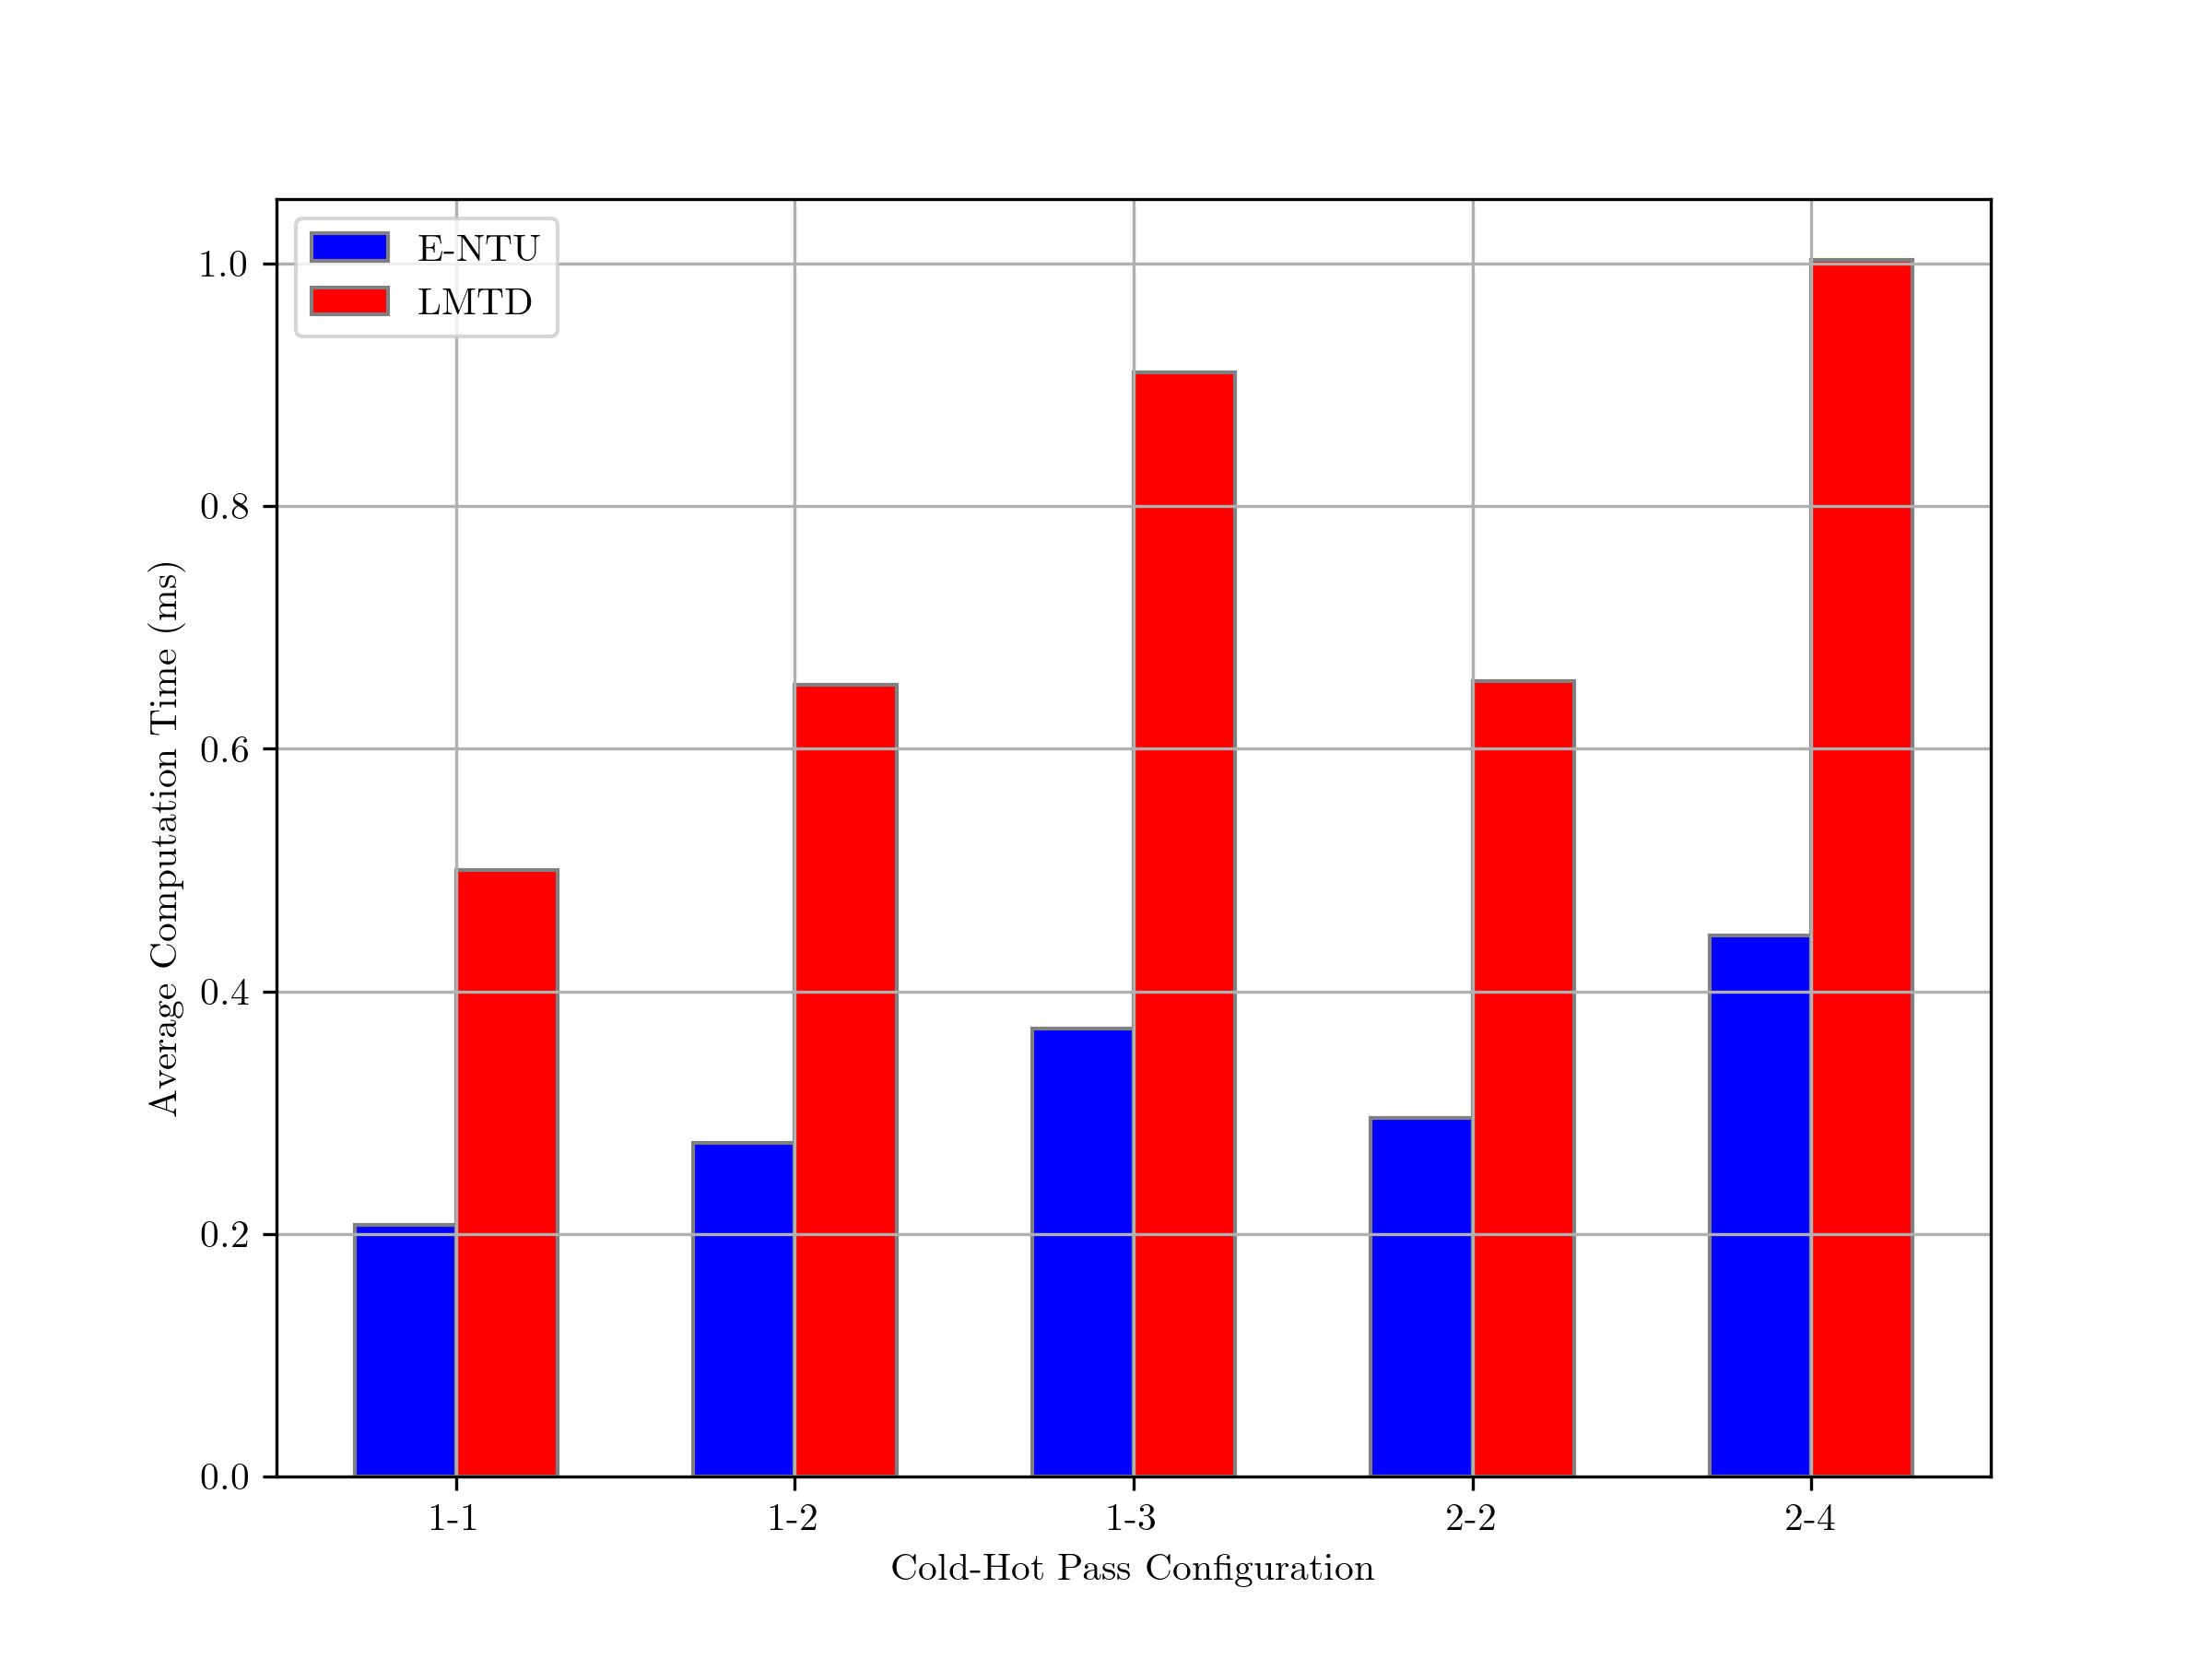
\includegraphics[width=0.8\textwidth]{entu_lmtd_speed.png}
  \caption{Calculation time for $\varepsilon$-NTU and LMTD methods for various heat exchanger configurations.}
  \label{fig:entu_lmtd_speed}
\end{figure}

\subsection{Comparison of Methods and Experimental Data}

Experimental data for previous designs was compared with our model to improve the accuracy.

\subsubsection{Hydraulic Analysis}

\begin{figure}[H]
  \centering
  \begin{subfigure}{.49\textwidth}
    \centering
    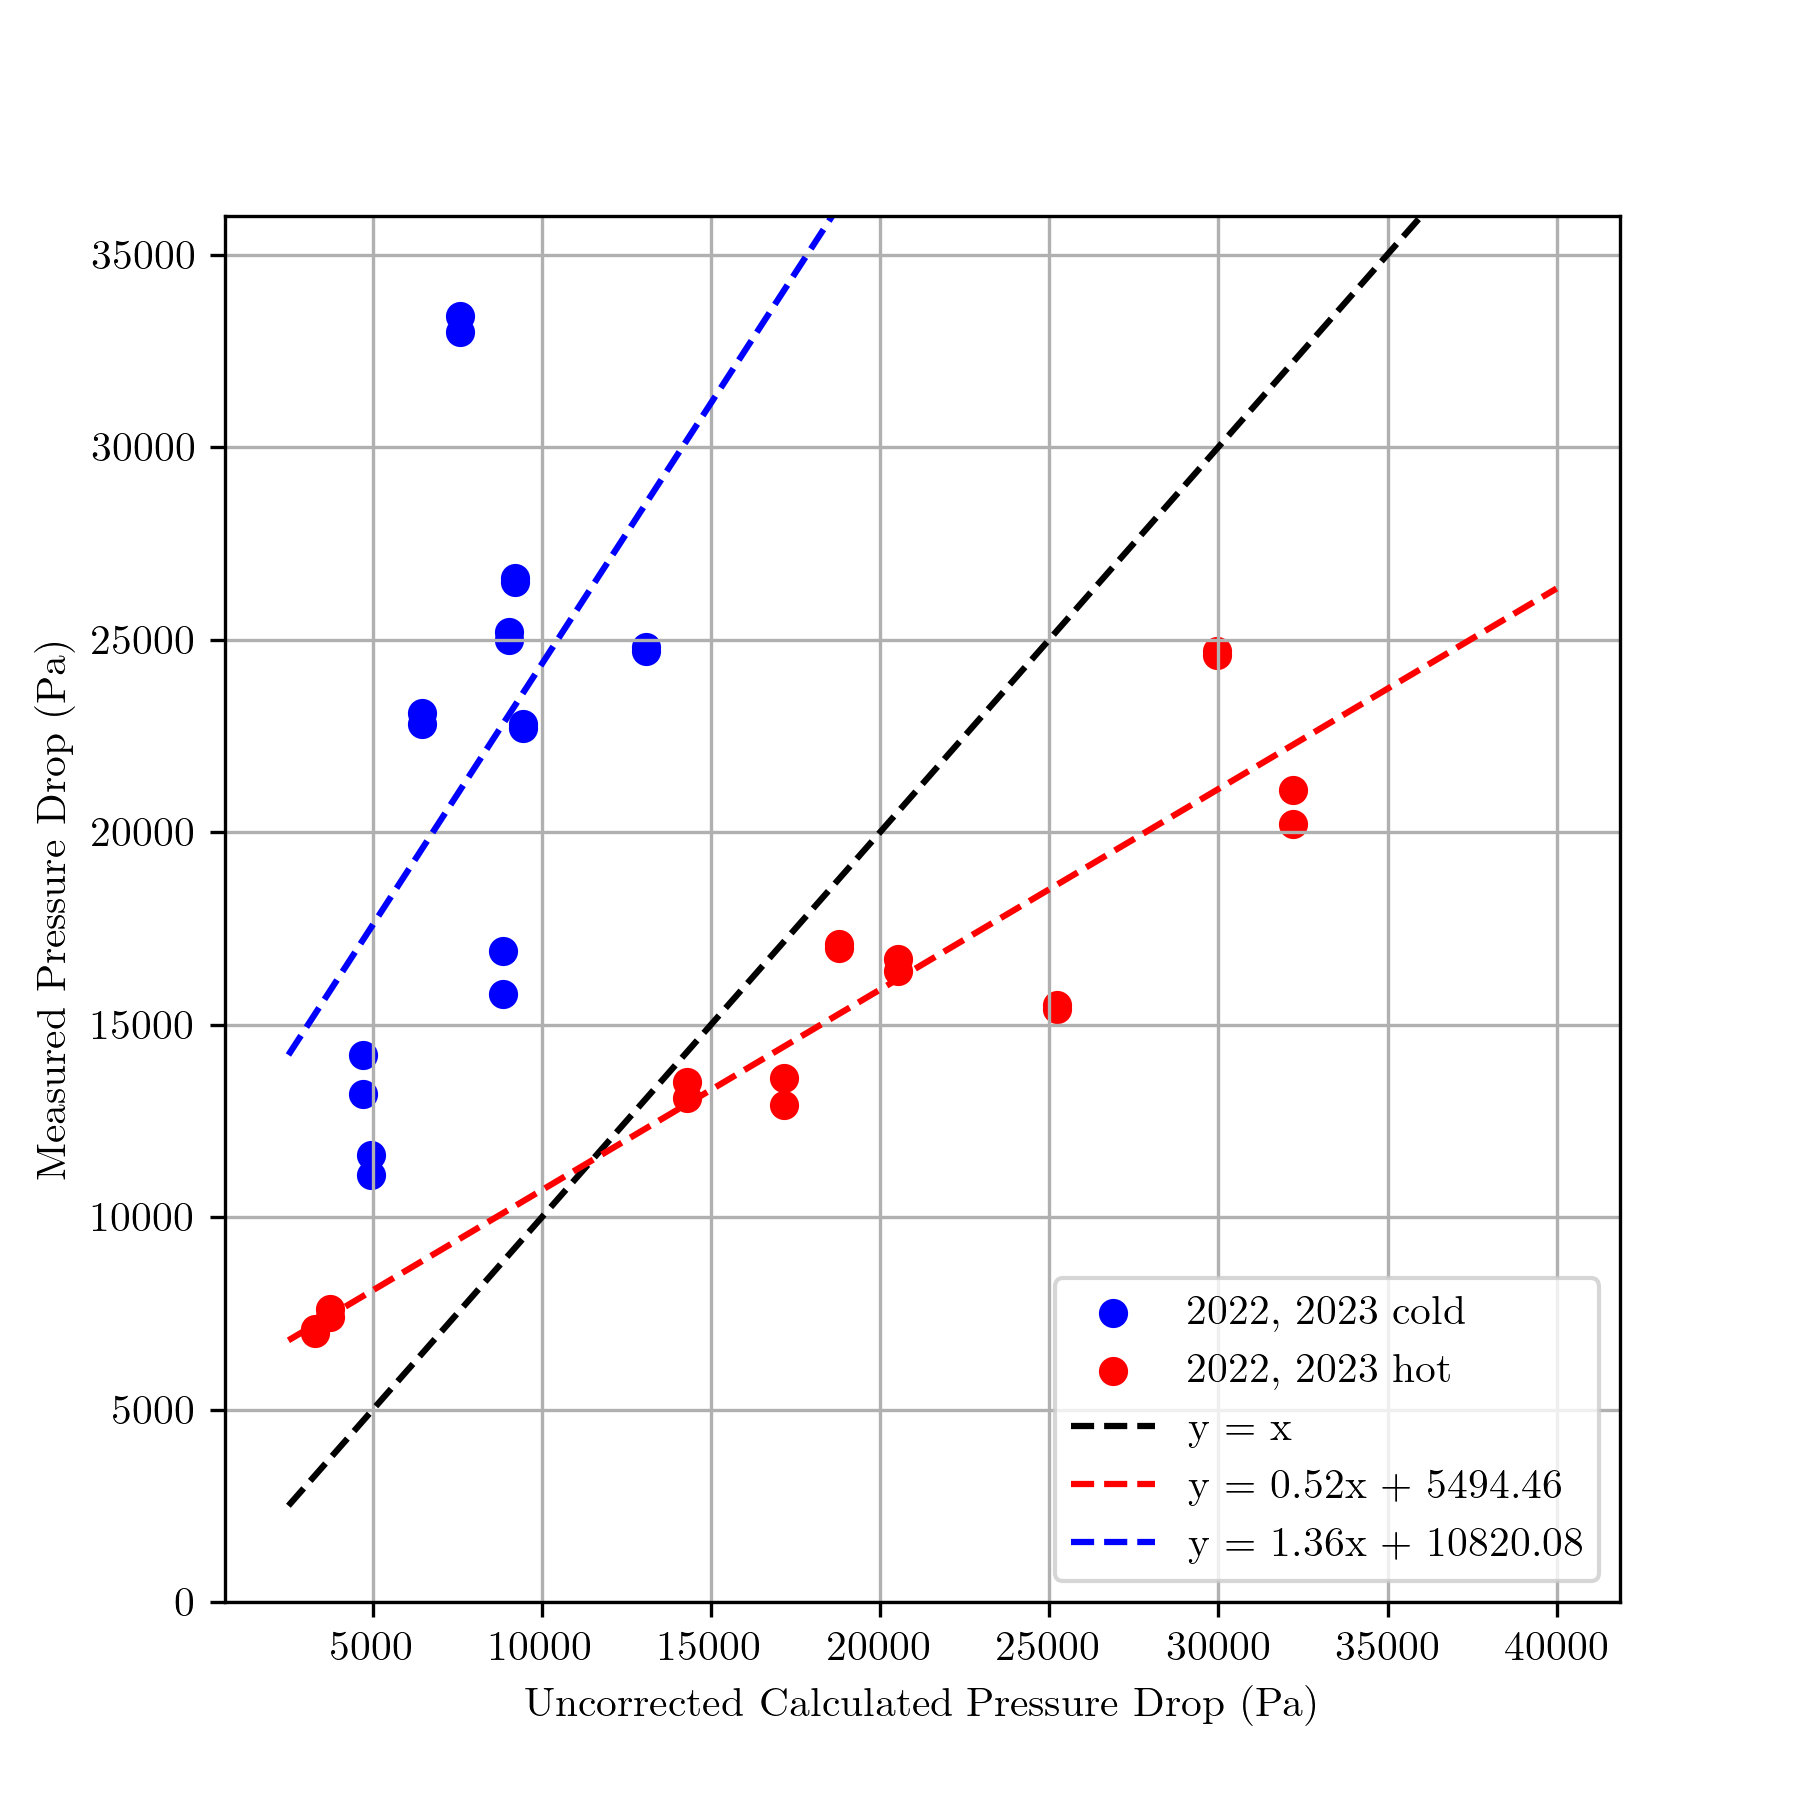
\includegraphics[width=0.99\textwidth]{dp_ucalc_vs_meas.png}
    \caption{Correction lines from 2022 and 2023 designs.}
    \label{fig:uncorrected_pressure_drops}
  \end{subfigure}
  \begin{subfigure}{.49\textwidth}
    \centering
    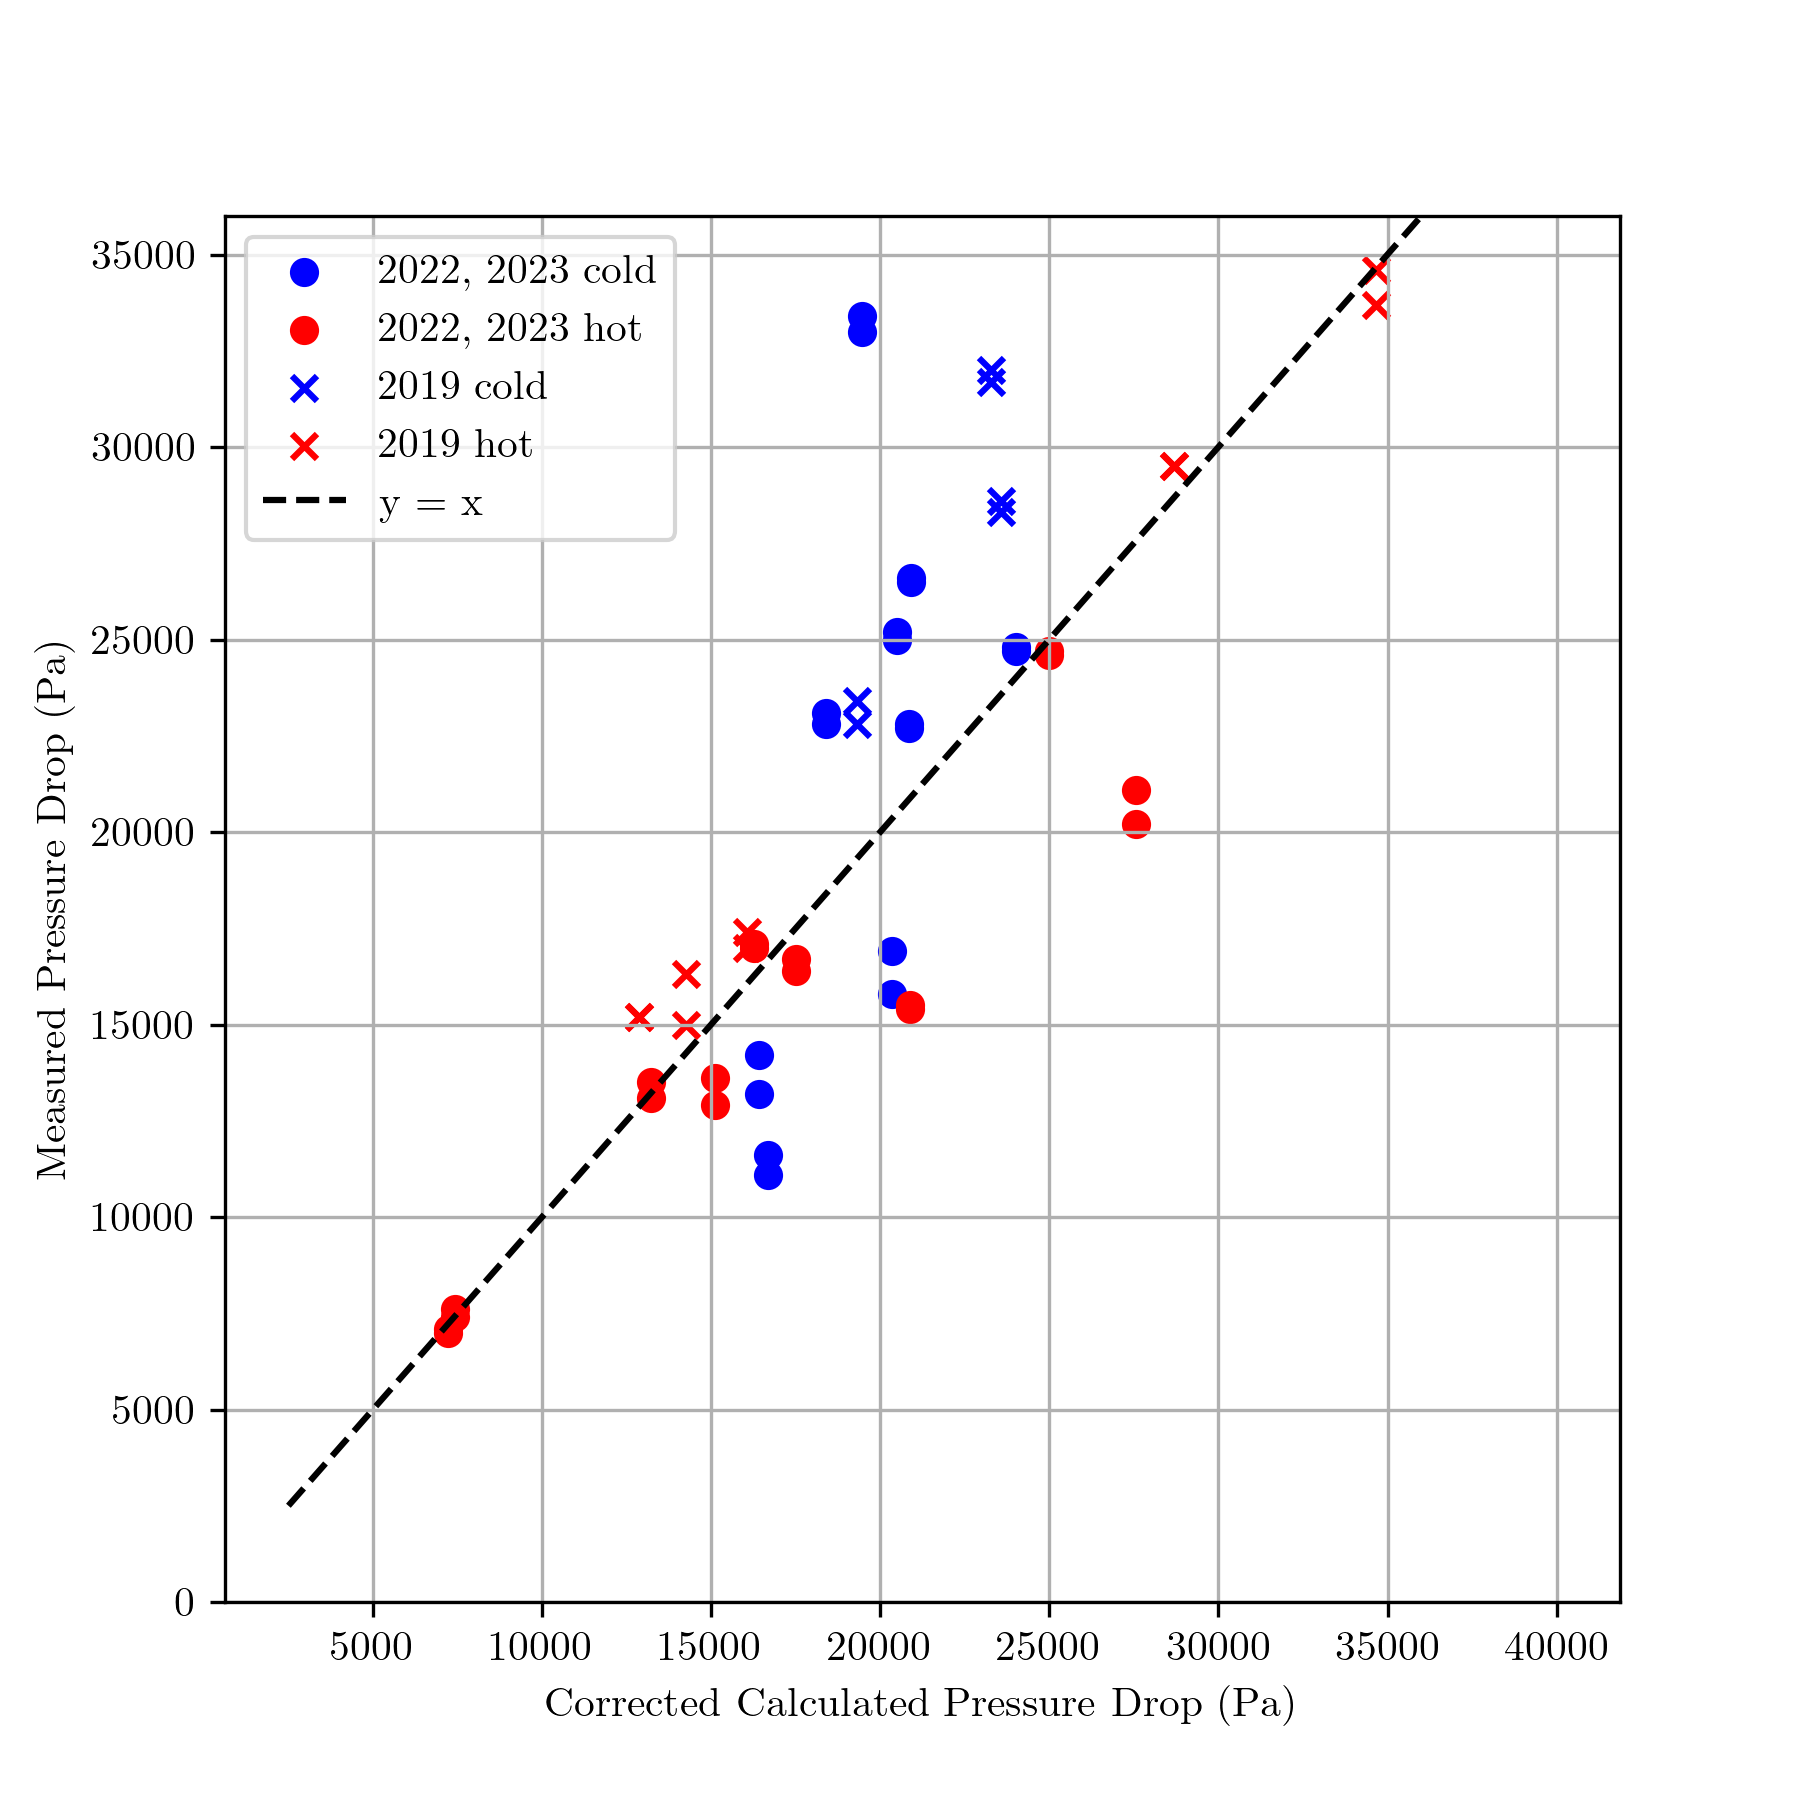
\includegraphics[width=.99\linewidth]{dp_ccalc_vs_meas.png}
    \caption{Applied correction on previous and new 2019 designs.}
    \label{fig:corrected_pressure_drops}
  \end{subfigure}
    
  \caption{Pressure drop calculated from measured mass flow rate compared to measured pressure drop.}
  \label{fig:pressure_drops}

\end{figure}

The correlation coefficients for hot and cold pressure drops are:  $\mathbf{0.93874}$ and $\mathbf{0.50926}$
This demonstrates that the model is more accurate at predicting the hot mass flow rate than the cold mass flow rate,
which is expected from Kerns simple method.
As shown, in the cold flow case, Kerns method significantly underestimates the pressure drop in the cold flow path, and in many cases, outside of the compressor characteristics.
The corrected pressure drop.

\subsubsection{$\varepsilon$-NTU and LMTD}

\subsubsection{Thermal}

\begin{figure}[H]
  \centering
  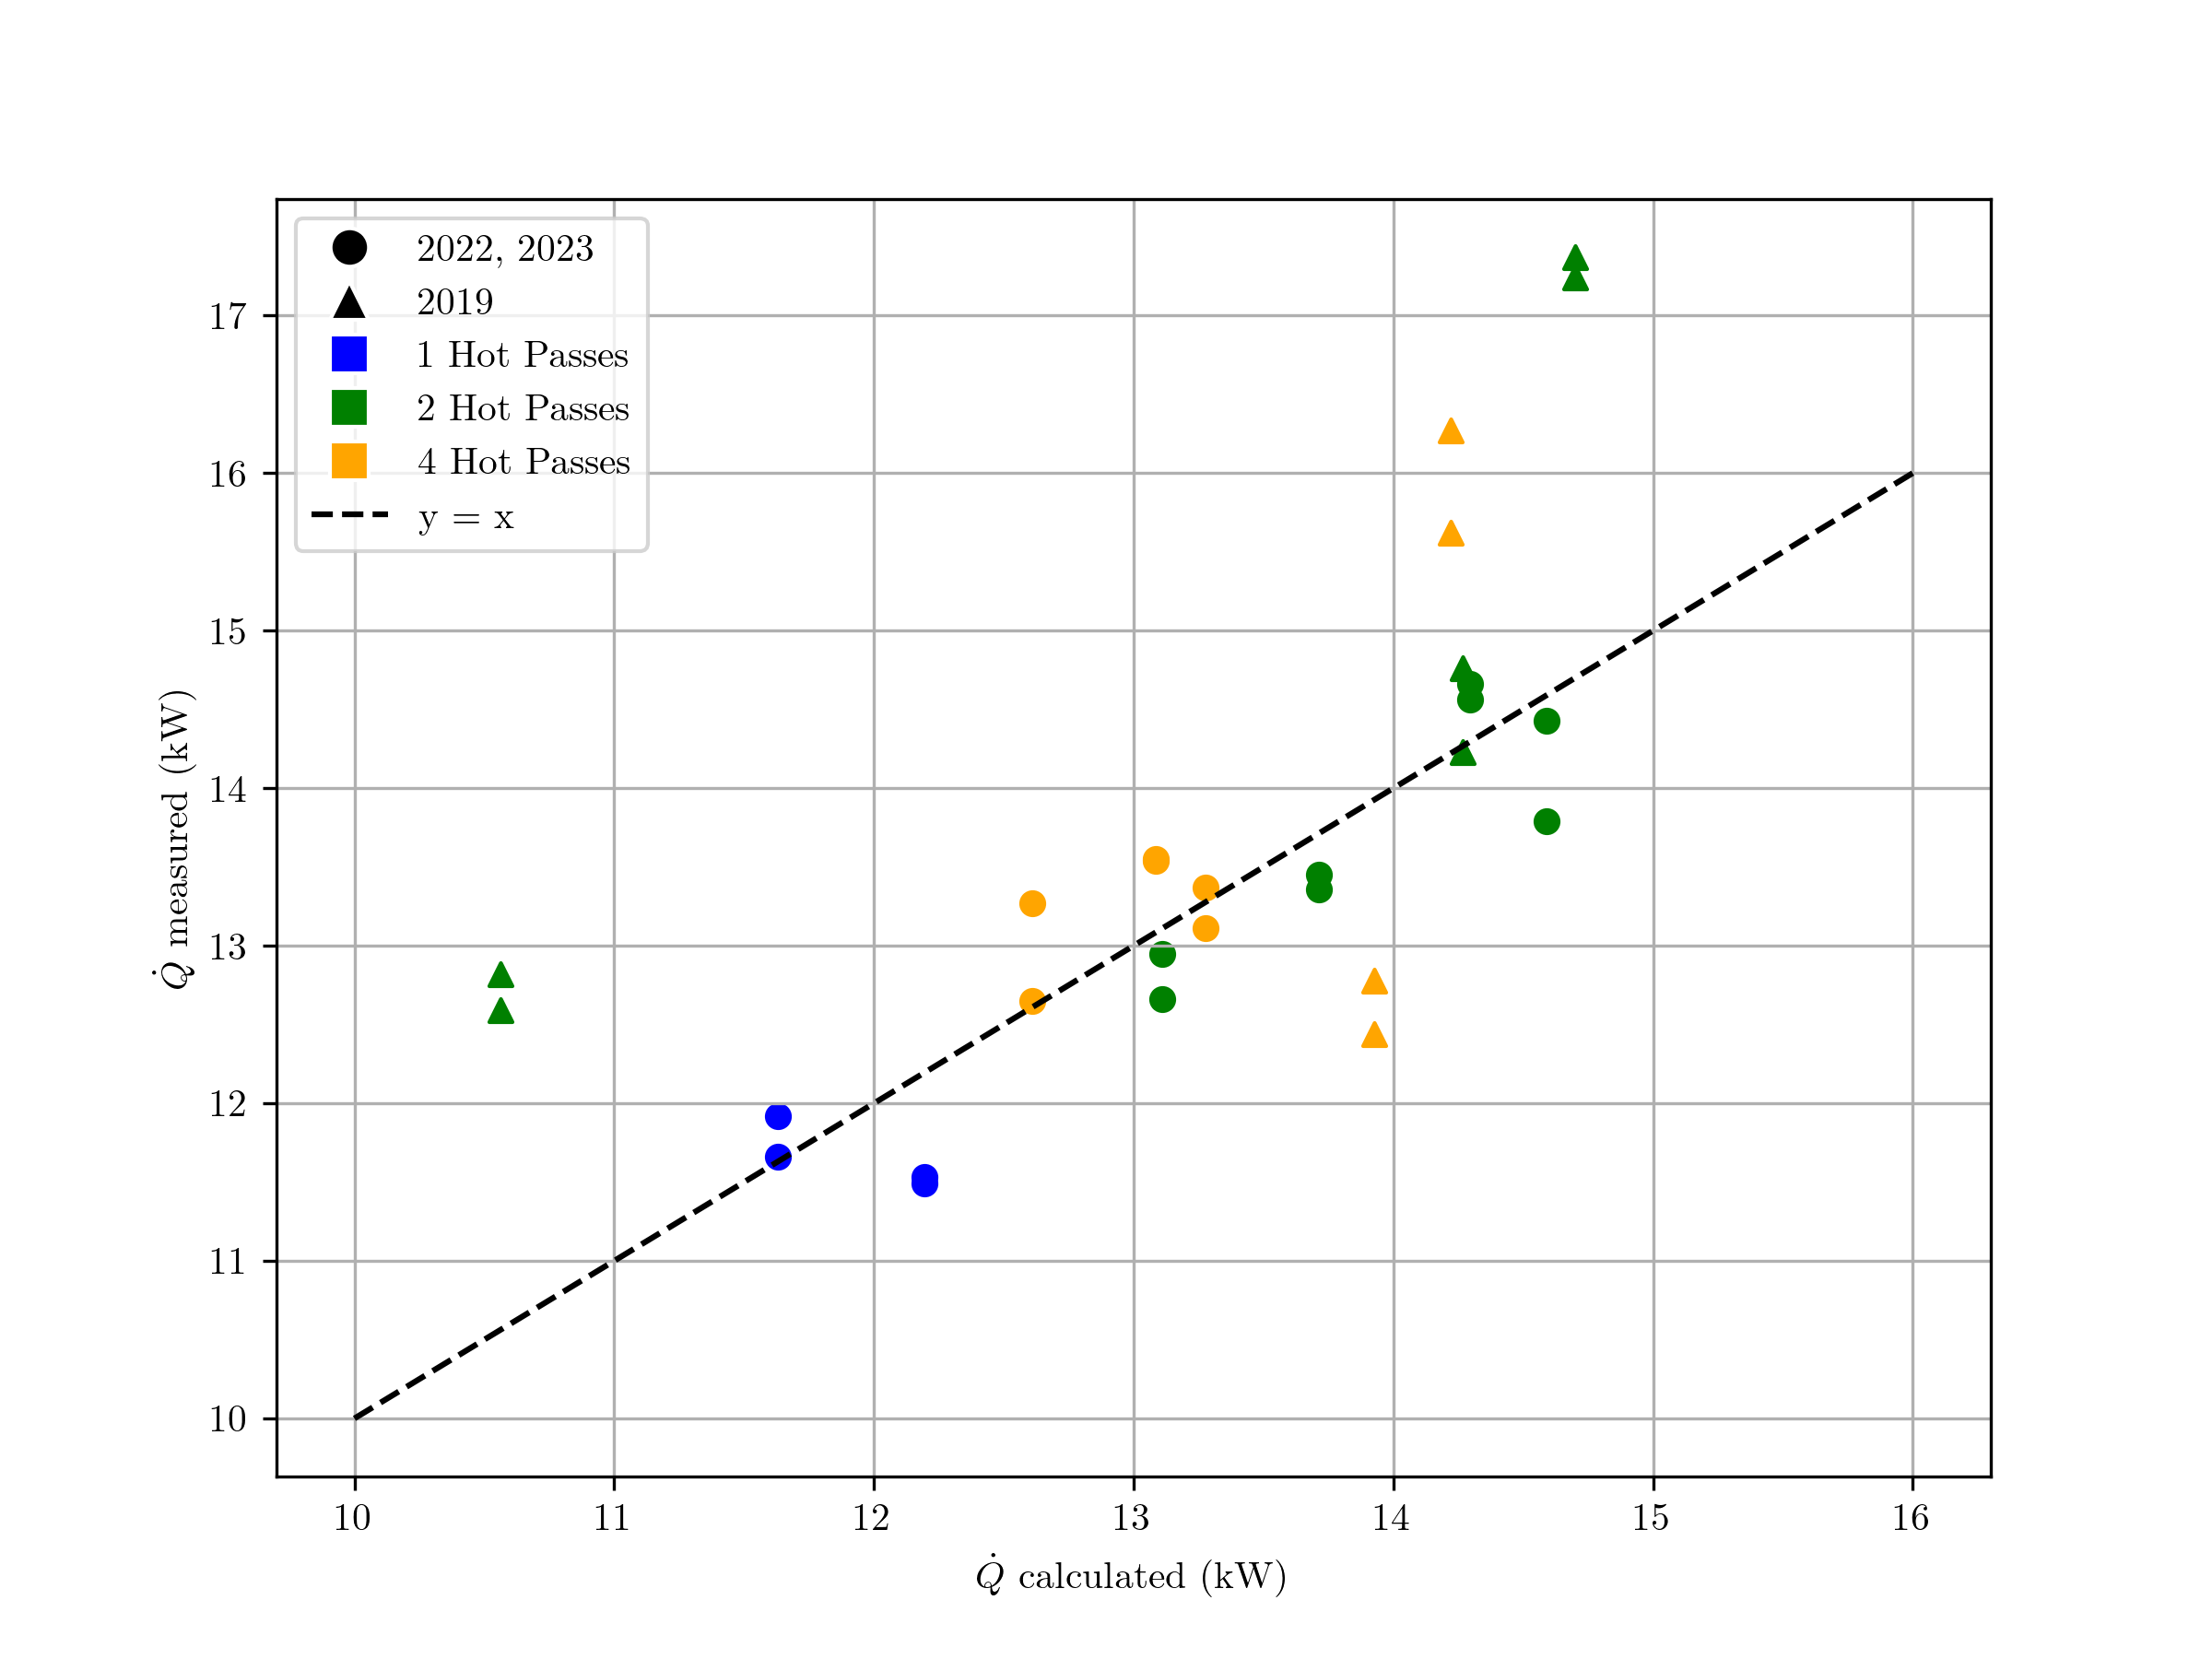
\includegraphics[width=0.8\textwidth]{Qdot_ccalc_vs_measured.png}
  \caption{Calculated against measured heat transfer rate.}
\end{figure}

\section{Optimization Problem}

The objective is to maximise the heat transfer rate $\dot{Q}$ subject to physical constraints.

\subsection{Constraints}

Many standard physical quantities are constrained to discrete values and standards, such as the number of tubes, baffles and pipe diameters.
For our design, we have the following constraints:
\begin{itemize}
  \item Total mass of the heat exchanger $M_{\text{total}} < 1.2$ Kg.
  \item Total length of the heat exchanger $L_{\text{total}} < 0.35$ m.
  \item Total length of the tubes $L_{\text{tubes}} < 3.5$ m.
  \item Tubes have outer and inner diameters, $d_{o} = 8$ mm, and $d_{i} = 6$ mm.
  \item Shell has inner diameter $D_{\text{shell}} = 64$ mm.
  \item Nozzles must 
\end{itemize}

Additional constraints were imposed to reduce the search space and simplify the problem.
The number of tubes was constrained to not decrease over the hot fluid path inside the heat exchanger.
This is thought to be a reasonable assumption because increasing the area at regions of smaller temperature difference increases overall heat transfer.
For example, if we were to decrease area then more heat transfer would occur in the first stage where there is a higher temperature difference, however there would be a significant reduction of heat transfer in the later stages.

\subsection{Design Parameters}

Significant simplifications were made to reduce the number of design parameters.
One such simplification was to assume that the tubes are packed as far away from each other as possible.
This means that the pitch can be calculated from the constrained geometry and number of tubes.

The search space for a given template with $p$ hot stages and $q$ cold stages is $p + q + 1$ dimensional.
This arises from the 1 dimensional length, number of tubes in each hot stage, and number of baffles in each cold stage.
The simplest design has 1 hot stage and 1 cold stage, and so the search space is 3 dimensional.

\subsection{Algorithms}
Three optimization algorithms were tested: Brute force, Sequential Least Squares Programming, and Simplicial Homology.
An unconstrained Nelder-Mead algorithm was also tested which had a cost value of infinity when constraints were violated but this did not reliably converge.
In an early version of the program, the brute force algorithm was both fast and robust at finding the global optimal design.
However, the introduction of a variable number of tubes and baffles in each stage increased the complexity $O(n^{p+q+1})$.

The Nelder-Mead algorithm

\subsection{Post Optimality Analysis}
% uncertainty quantification?

In reality there is a large uncertainty in the calculated values due to assumptions and empirical relations.


\section{Software}

\subsection{Implementation}

The Python application used PyQt6 and matplotlib for the GUI. The calculations were done using NumPy and SciPy libraries.
The software tool allows the user to interactively change the design parameters for a wide range of heat exchanger configurations.
Calculated values are displayed in real-time and the user can compare the performance of different designs.
When the optimiser is started it will attempt to find the optimal design for the number of stages and tube patterns set.
After an optimal solution is found, the design is loaded into the GUI for manual inspection and comparison with other designs.

\subsection{Design}
The software features object oriented design with classes for the heat exchanger and fluid path components.
The structure is designed to be easily extendable with new components and optimization thread workers.
Seperate optimization threads are used to prevent the GUI from freezing during long calculations.

The graphical user interface is designed to be intuitive and user friendly. A log dispays optimization progress, warning and error messages. There is also a diagram of the heat exchanger which helps
the user visualise the flow path of multi-stage designs.

\begin{figure}[H]
  \centering
  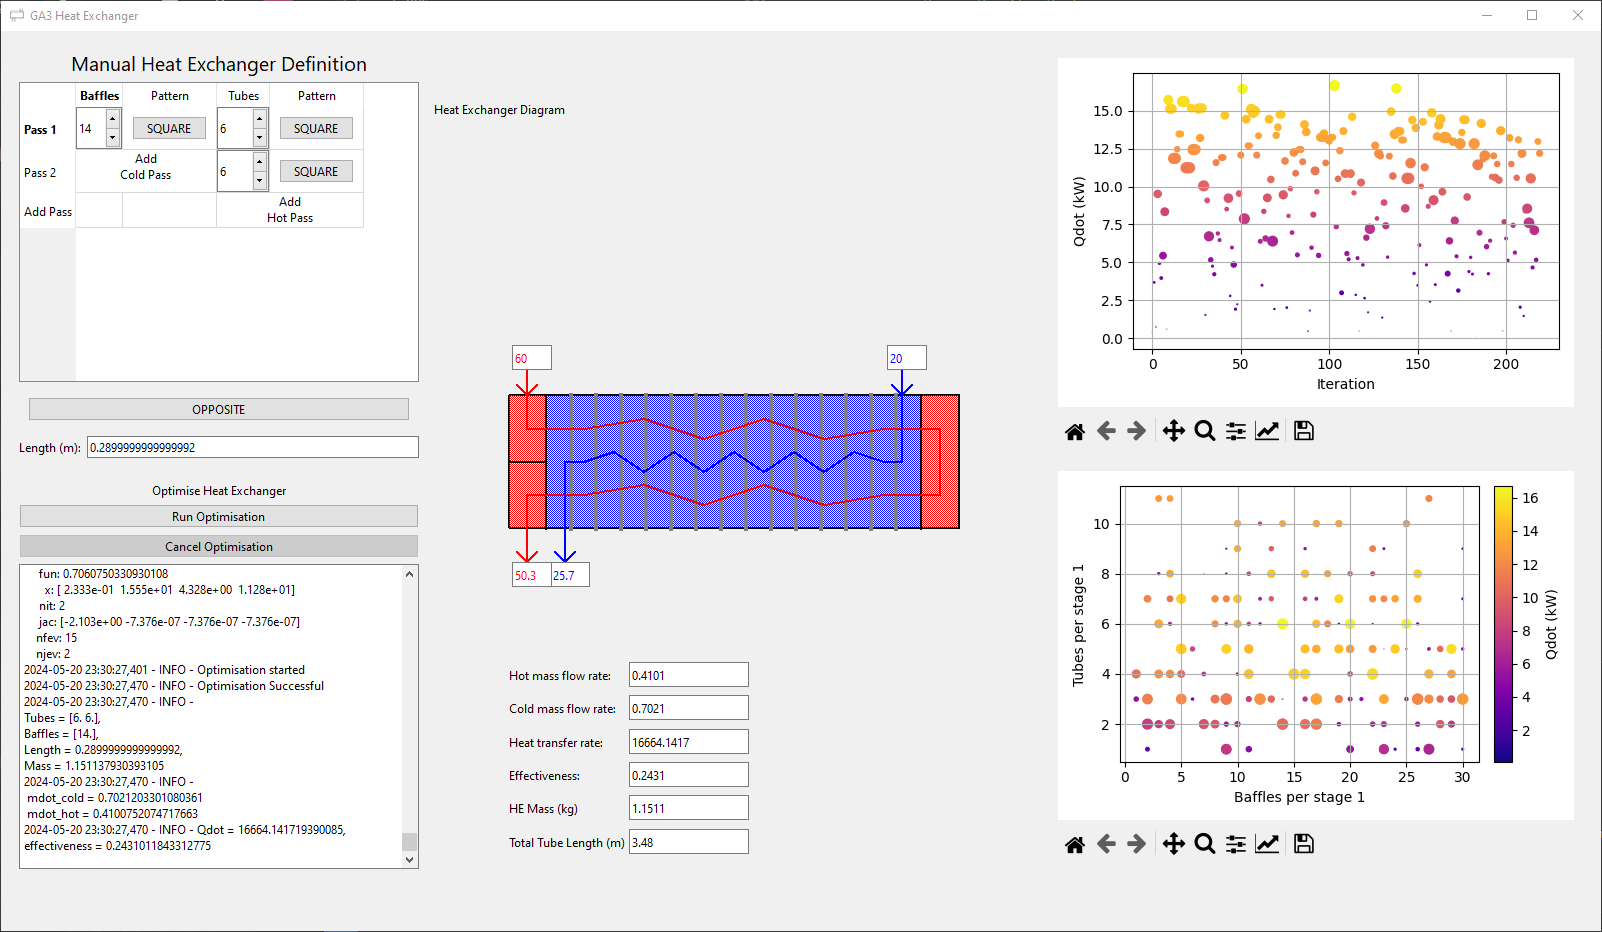
\includegraphics[width=0.6\textwidth]{software.png}
  \caption{Screenshot of the software tool.}
  \label{fig:software}
\end{figure}

\subsection{Best Designs from Constraints}
% challenging to visualise higher dimensional spaces
% I'm not as big as a fan of 3D plots as I used to be - they're harder to interpret than colour maps
Configurations with more stages provide additional complexity in the manufacturing process.




\section{Discussion}

\subsection{Comparison of $\varepsilon$-NTU and LMTD Methods}



\section{Conclusion}


\newpage
\section{Appendix}

\begin {lstlisting}[language=Python]

\end{lstlisting}


% bibliography
\newpage
\begin{thebibliography}{9}

\bibitem{handout}
  G. Vinnicombe,
  \emph{Inverted Pendulum Lab Handout}.
  University of Cambridge,
  2022.

\bibitem{feedback_control_of_dynamic_systems}
  G. F. Franklin, J. D. Powell, A. Emami-Naeini,
  \emph{Feedback Control of Dynamic Systems}.
  Pearson,
  2015.

\bibitem{non_linear_systems}
  H. K. Khalil,
  \emph{Nonlinear Systems}.
  Pearson,
  2002.

\bibitem{modern_control_systems}
  R. C. Dorf, R. H. Bishop,
  \emph{Modern Control Systems}.
  Pearson,
  2016.

\end{thebibliography}

\end{document}